\documentclass[11pt]{report}
\usepackage[utf8]{inputenc}
\usepackage[T1]{fontenc}
\usepackage[top=2cm, bottom=2cm, left=2cm, right=2cm]{geometry}
\usepackage{setspace}
\usepackage{graphicx}
\usepackage{float}
\usepackage{amsmath}
\usepackage{stmaryrd}
\usepackage{titlesec}
\usepackage{rotating}
\usepackage{alltt}
\usepackage{fancyvrb}
\usepackage{verbatimbox}
\usepackage{lipsum}
\titleformat{\chapter}[hang]{\bf\huge}{\thechapter}{2pc}{}

%-------------------------------------------------------
\let\oldabstract\abstract
\let\oldendabstract\endabstract
\makeatletter
\renewenvironment{abstract}
{\renewenvironment{quotation}%
               {\list{}{\addtolength{\leftmargin}{3em} % change this value to add or remove length to the the default
                        \listparindent 1.5em%
                        \itemindent    \listparindent%
                        \rightmargin   \leftmargin%
                        \parsep        \z@ \@plus\p@}%
                \item\relax}%
               {\endlist}%
\oldabstract}
{\oldendabstract}
\makeatother

\makeatletter
\newcommand{\verbatimfont}[1]{\renewcommand{\verbatim@font}{\normalfont#1}}
\makeatother

\begin{document}
\begin{center}

\includegraphics[scale = 1]{index.png}
\end{center}

\pagestyle{empty}
\vspace*{\stretch{8}}


\centerline{\textbf{\Huge Parser Documentation}}
\bigbreak\bigbreak
\bigbreak\bigbreak

\centerline{ {\Large Estelle Alauzy}}
\vspace*{\stretch{1}}
\centerline{ {\Large  Chervin Amirkaveh}}


 \vfill
 \vspace*{\stretch{10}}
\centerline{\large June 2019}
\vspace*{\stretch{1}}






%%%%%%%%%%%%%%%%%%%%%%%%%%%%%%%%%%%%%%%%%%%%%%%%%%%%%%%%%%%%%%%%%%%%%%%%%%%%
%%%%%%%%%%%%%%%%%%%%%%%%%%%%%%%%%%%%%%%%%%%%%%%%%%%%%%%%%%%%%%%%%%%%%%%%%%%%
\newpage
\centerline{\textbf{\Huge Grammar : Backus-Naur form (BNF)}}
\vspace*{3pt}
\vspace*{3pt}
\begin{Verbatim}[fontfamily=textsf]
Program ::= FuncDecla Program
            | VariableDecla Program
            | FuncDecla CallMain
            | VariableDecla CallMain
\end{Verbatim}
\vspace*{3pt}

\begin{verbnobox}[\normalfont]
FuncDecla ::= func FuncType name (Parameters) Body
\end{verbnobox}
\vspace*{3pt}

\begin{verbnobox}[\normalfont]
Parameters ::= Typ identifier | Typ identifier , Parameters
\end{verbnobox}
\vspace*{3pt}

\begin{verbnobox}[\normalfont]
Body ::= { Instruction } | { VariableDeclas ; Instruction }
\end{verbnobox}
\vspace*{3pt}

\begin{verbnobox}[\normalfont]
VariableDecla ::= Typ identifier | Typ ( TupleDecla )
\end{verbnobox}
\vspace*{3pt}

\begin{verbnobox}[\normalfont]
TupleDecla ::= identifier | identifier , TupleDecla
\end{verbnobox}
\vspace*{3pt}

\begin{verbnobox}[\normalfont]
VariableDeclas ::= VariableDecla VariableDeclas | VariableDecla
\end{verbnobox}
\vspace*{3pt}

\begin{verbnobox}[\normalfont]
Instruction ::= Bintruction | Binstruction Instruction
\end{verbnobox}
\vspace*{3pt}

\begin{verbnobox}[\normalfont]
Binstruction ::= Expression = Expression 
                 | Expression = call name ( Expression )
                 | call name ( Expression )
                 | Expression = receive ( identifier )
                 | send ( identifier , Expression )
                 | if ( Expression ) { Instruction } else { Instruction }
                 | let Expression = Expression in { Instruction }
                 | while ( Expression ) { Instruction }
                 | choose { Choices }
                 | spawn ( name , Expression )
                 | Expression = new ( Typ )
                 | return Expression
                 | noop
\end{verbnobox}
\vspace*{3pt}

\begin{verbnobox}[\normalfont]
Choices ::= Prefix -> { Instruction } Choices | Prefix -> { Instruction }
\end{verbnobox}
\vspace*{3pt}

\begin{verbnobox}[\normalfont]
Prefix ::= tau
         | | send ( identifier , Expression )
         | | Expression = receive ( identifier )
         | | Expression = new ( Typ )
         | | spawn ( name , Expression )
\end{verbnobox}
\vspace*{3pt}

\begin{verbnobox}[\normalfont]
Expression ::= - Expression
               | head ( Expression )
               | tail ( Expression )
               | odd ( Expression )
               | even ( name , Expression )
               | Expression + Expression
               | Expression - Expression
               | Expression || Expression
               | Expression * Expression
               | Expression / Expression
               | Expression && Expression
               | Expression == Expression
               | Expression < Expression
               | Expression > Expression
               | let Expression = Expression in ( Expression )
               | if ( Expression ) { Expresssion } else { Expression }
               | ( ExpressionSeq )
               | Value
               | identifier
\end{verbnobox}
\vspace*{3pt}

\begin{verbnobox}[\normalfont]
ExpressionSeq ::= Expression | Expression , ExpressionSeq
\end{verbnobox}
\vspace*{3pt}

\begin{verbnobox}[\normalfont]
Constant ::= number
             | ' char '
             | " string "
             | true
             | false
\end{verbnobox}
\vspace*{3pt}

\begin{verbnobox}[\normalfont]
Value ::= Constant | { ValueSeq }
\end{verbnobox}
\vspace*{3pt}

\begin{verbnobox}[\normalfont]
ValueSeq ::= Value | Value , ValueSeq
\end{verbnobox}
\vspace*{3pt}

\begin{verbnobox}[\normalfont]
Typ ::= int
      | boolean
      | string
      | char
      | channel
      | list [ Typ ]
      | ( Types ) 
\end{verbnobox}
\vspace*{3pt}

\begin{verbnobox}[\normalfont]
Types ::= Typ | Typ , Types
\end{verbnobox}
\vspace*{3pt}

\begin{verbnobox}[\normalfont]
FuncType ::= void | Typ
\end{verbnobox}
\vspace*{3pt}

\begin{verbnobox}[\normalfont]
CallMain ::= start name ( Expression )
\end{verbnobox}
\vspace*{3pt}

\newpage
\centerline{\textbf{\Huge Examples}}
\vspace*{3pt}
\vspace*{20pt}
Communicating and mobile systems : the $\pi$-calculus - Robin Milner : The mobile phones system

\begin{center}
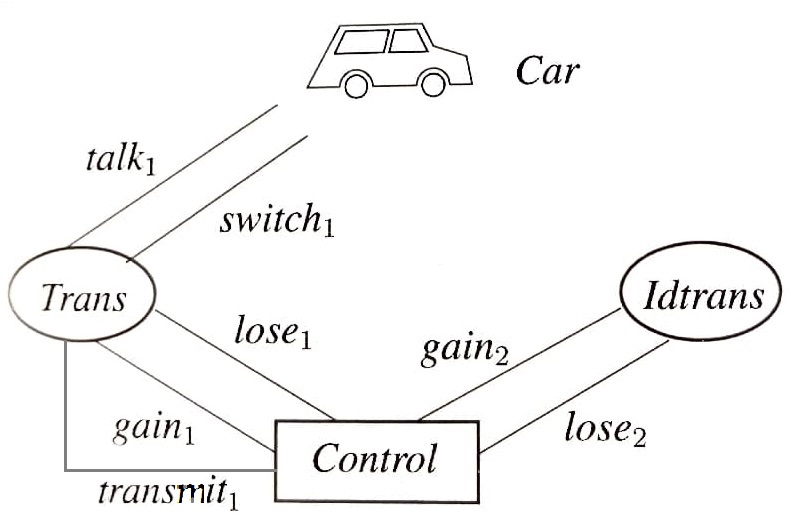
\includegraphics[scale = 0.5]{mobile-phone-system.jpg}
\end{center}
Add the Description of the example from the book p-82

To allow the control to know when it needs to act we add an other channel between Control and Trans named transmit1. This channel transmit the message received by Trans since Car. This message is an integer which represents the position of the car. We arbitrarily decide the position when links between the Trans and the car must be switch to the other trans : Idtrans. So, when the position is greater than the threshold the Control tells to Trans to lose the car and to IdTrans to gain the car.

\end{document}
